Tam, kad nustatyti ar verta formaliai įrodyti sukurtą algoritmą buvo atlikti empiriniai bandymai, kurie skirti ištirti algoritmo korektišką veikimą ir efektyvumą. Šiems bandymams atlikti buvo įgyvendintas sukurtas algoritmas, modulis, generuojanti tinklus, ir modulis, kuris atlieka bandymus su tinklus generuojančio modulio rezultatais. Su bandymus atliekančio modulio rezultatais yra atliekami statistiniai skaičiavimai.

\subsection{Tinklus generuojantis modulis}

Šiame darbe reikia ištirti kuo įvairesnius tinklus, iš kurių parametrų būtų paprasta sukonstruoti regresinius modelius. Tad tinklus generuojantis modulis turi generuoti tinklus $N_i = \{V_{N_i}, E_{N_i}, u{N_i}\}$, kurių parametrai tenkintų šias sąlygas:
\begin{itemize}
	\item Viršūnių aibių  $V_{N_i}$ dydžių aibės $SV$ augimo greitis būtų linijinis ir $SV$ turi būti baigtinė.
	\item Kiekvieną kartą generuojant tinklą $N_i$ yra tikimybė sugeneruoti jungų tinklą.
	\item Sugeneruotų tinklų aibėje egzistuoja tinklai su skirtingais viršūnių aibių dydžiais ir vidutiniu galimų briaunų skaičiumi. Vidutinis galimų briaunų skaičius yra apskaičiuojamas $SE_a = \frac{SE_{max} + SE_{min}}{2}$, kur  $SE_{max}$ yra maksimalus galimų briaunų skaičius, o $SE_{min}$ - minimalus galimų briaunų skaičius.
	\item Sugeneruotų tinklų aibėje egzistuoja tinklai su skirtingais viršūnių aibių dydžiais ir vidutiniškai mažesniu briaunų skaičiumi negu vidutinis galimų briaunų skaičius.  Tinklo briaunų skaičius yra laikomas vidutiniškai mažesniu negu vidutinis galimų briaunų skaičius, jei tenkinama sąlyga: $SE_{a_{min}} = \frac{SE_a + SE_{min}}{2}$, kur $SE_a$ yra vidutinis galimų briaunų skaičius, o $SE_{min}$ - minimalus galimų briaunų skaičius.
	\item Sugeneruotų tinklų aibėje egzistuoja tinklai skirtingais viršūnių aibių dydžiais ir vidutiniškai didesniu briaunų skaičiumi negu vidutinis galimų briaunų skaičius.  Tinklo briaunų skaičius yra laikomas vidutiniškai didesniu negu vidutinis galimų briaunų skaičius, jei tenkinama sąlyga: $SE_{a_{max}} = \frac{SE_a + SE_{max}}{2}$, kur $SE_a$ yra vidutinis galimų briaunų skaičius, o $SE_{max}$ - maksimalus galimų briaunų skaičius.
\end{itemize}
Žinant, kad minimalus galimų briaunų skaičius tinkle yra $SE_{min}(SV_i)  = SV_i - 1$, o maksimalus galimų briaunų skaičius tinkle yra $SE_{max}(SV_i) = SV_i \times (SV_i - 1)$, kur $SV_i$ yra tinko viršūnių skaičius, tai gauname, kad  $SE_{a}(SV_i) =\frac{SV_i^2 - 1}{2}$, $SE_{a_{min}}(SV_i)  = \frac{SV_i^2 + 2 \times SV_i - 3}{4}$ ir $SE_{a_{max}}(SV_i) = \frac{3 \times SV_i^2 - 2 \times SV_i - 1}{4}$.

Tad tinklus generuojantis modulis sugeneruoja tinklų $N_i = \{V_{N_i}, E_{N_i}, u{N_i}\}$ aibę A. Aibėje A yra 10 poaibių $A'_j$, kurių tinklų viršūnių aibių $V_{N_i}$ dydžiai $SV_i$ yra lygūs. Tad kiekvienas poaibis  $A'_j$ turi skirtingą dydį  $SV_j$. Modulis sugeneruoja poaibius $A'_j$ su šiais $SV_j = 10 \times j : j = 1 .. 10$. Kiekviename poaibyje $A'_j$ yra po 3 poaibius $A''_j$, kuriuose yra po 10 tinklų $N_i$, kurių briaunų aibių $E_{N_i}$ dydžiai yra lygūs. Tad kiekvienas poaibis  $A''_j$ turi skirtingą dydį  $SE_j$. Modulis sugeneruoja poaibius $A''_j$ su šiais  $SE_j : SE_{a}(SV_i), SE_{a_{min}}(SV_i) , SE_{a_{max}}(SV_i)$.

\subsection{Bandymus atliekantis modulis}

Šiame darbe buvo sukurtas modulis ,kuris atlieka bandymus su kiekvienu tinklu, kurį sugeneravo tinklus generuojantis modulis. Šių bandymų metu yra skaičiuojamas briaunų panaudotų skaičiavimuose skaičius. Šio bandymo rezultatai yra masyvai INCORRECT, ACTION, $Algorithm_{\{T\}}$ ir $Test_{\{T\}}$, kur T yra kiekvieno dinaminio tinklo operacijos tipas. Šio bandymo eiga su tinklu NETWORK:

\begin{enumerate}
	\item Apskaičiuojamas tinklo NETWORK maksimalus srautas ACTUAL, naudojant sukurto algoritmo įgyvendinimą.
	\item Apskaičiuojamas tinklo NETWORK maksimalus srautas EXPECTED, naudojant modifikuotą Fordo Fulkersono algoritmą.
	\item Jei $ACTUAL \neq EXPECTED$, tai į masyvą INCORRECT įdedama grupė G, o į masyvą ACTION reikšmė \textit{INIT}.
	\item Su kiekvienu dinaminio tinklo operacijos tipu TYPE yra atliekami šie veiksmai:
	\begin{enumerate}
		\item Tinklui NETWORK atliekama operacija TYPE.
		\item Apskaičiuojamas tinklo NETWORK maksimalus srautas ACTUAL, naudojant sukurto algoritmo įgyvendinimą. Į $Algorithm_{TYPE}$ įdedamas skaičiavime panaudotų briaunų skaičius.
		\item Apskaičiuojamas tinklo NETWORK maksimalus srautas EXPECTED, naudojant modifikuotą Fordo Fulkersono algoritmą. Į $Test_{TYPE}$ įdedamas skaičiavime panaudotų briaunų skaičius.
		\item Jei $ACTUAL \neq EXPECTED$, tai į masyvą INCORRECT įdedamas tinklas NETWORK, o į masyvą ACTION įdedamas TYPE.
	\end{enumerate}

\end{enumerate}

\subsection{Statistiniai skaičiavimai ir jų rezultatai}

Naudojantis atliktų bandymų rezultatu, INCORRECT ir ACTION masyvais, buvo nustatyta, kad iš 300 apskaičiuotų tinklų tinklo N maksimalus srautas buvo nekorektiškai apskaičiuotas. Tinklo Nviršūnių aibių dydis yra 10, o briaunų skaičius yra vidutiniškai mažesnis už vidutinį galimų briaunų skaičių. Ištyrus tinklą N buvo nustatyta, kad grupavimo funkcija , jį sugrupavo taip, kad algoritmas dėl savo trūkumo, aprašyto skyriuje 1.5, negalėjo teisingai apskaičiuoti maksimalaus srauto. Todėl taip pat buvo nekorektiškai apskaičiuoti šių tinklų maksimalūs srautai po kiekvieno pokyčio. Tačiau žinant, kad maksimalus srautas buvo nekorektiškai apskaičiuotas inicializavimo fazėje, tai galima teigti, kad yra nežinoma ar algoritmas po kiekvieno pokyčio apskaičiavo maksimalų srautą korektiškai.

Atliktų bandymų rezultatai, masyvai $Algorithm_{\{T\}}$ ir $Test_{\{T\}}$, yra pateikti prieduose poskyryje Atliktų bandymų rezultatai \ref{experiment:add}, \ref{experiment:remove} ir \ref{experiment:update}. Naudojantis šiais masyvais buvo sukurti grafikai \ref{plot:vav}, \ref{plot:vae}, \ref{plot:vrv}, \ref{plot:vre}, \ref{plot:vue}, \ref{plot:eav}, \ref{plot:eae}, \ref{plot:erv}, \ref{plot:ere} ir \ref{plot:eue}, kurie yra pagalbinė priemonė algoritmų efektyvumų palyginimui.

\begin{figure}[H]
	\caption{Skaičiavime panaudotų briaunų skaičius po viršūnės pridėjimo tinklo viršūnių skaičiaus kontekste}
	\centering
	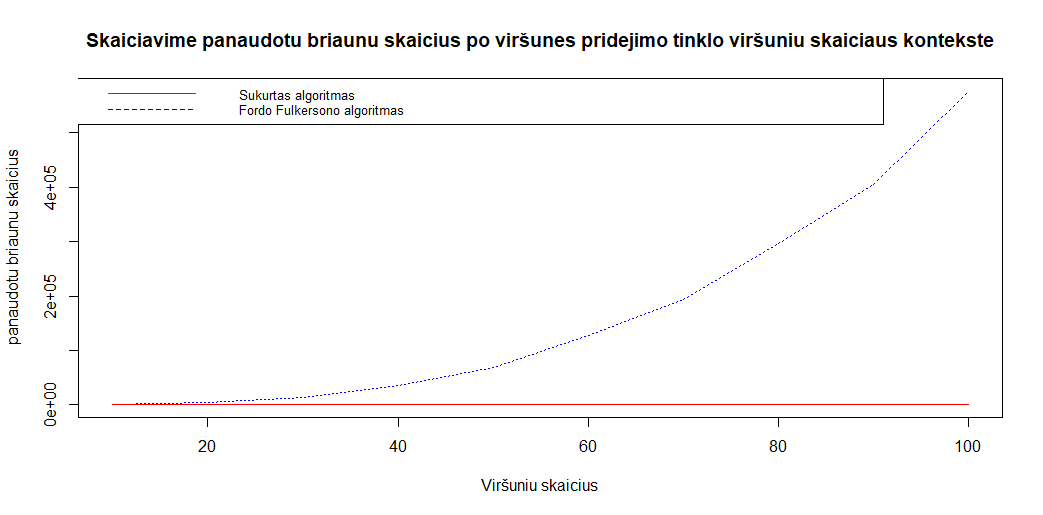
\includegraphics[width=\textwidth]{img/vav.png}
	\label{plot:vav}
\end{figure}
\begin{figure}[H]
	\caption{Skaičiavime panaudotų briaunų skaičius po briaunos pridėjimo tinklo viršūnių skaičiaus kontekste}
	\centering
	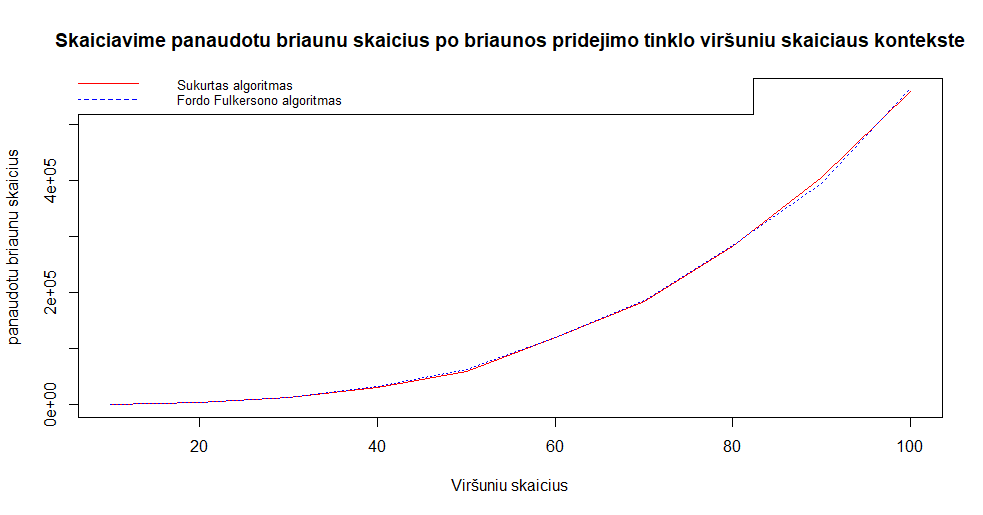
\includegraphics[width=\textwidth]{img/vae.png}
	\label{plot:vae}
\end{figure}
\begin{figure}[H]
	\caption{Skaičiavime panaudotų briaunų skaičius po viršūnės atėmimo tinklo viršūnių skaičiaus kontekste}
	\centering
	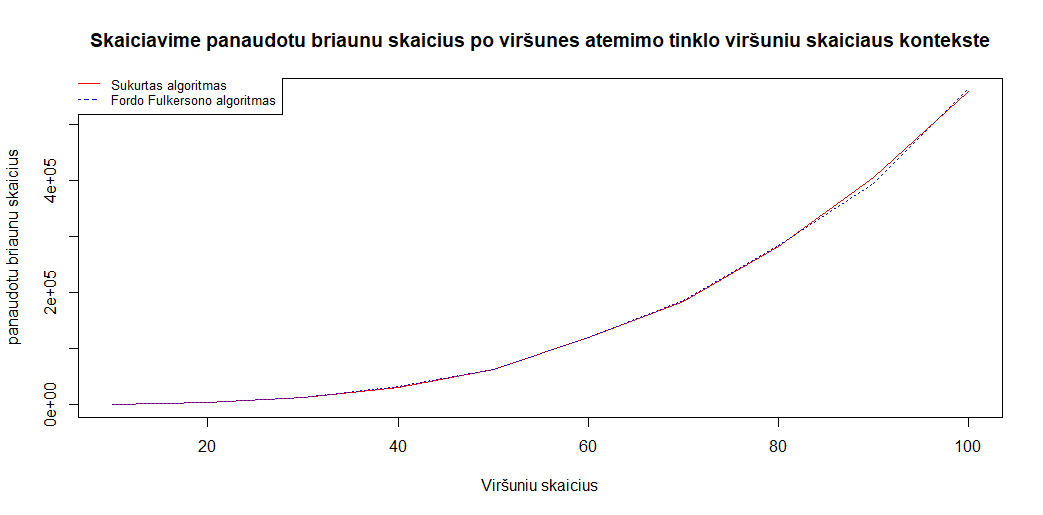
\includegraphics[width=\textwidth]{img/vrv.png}
	\label{plot:vrv}
\end{figure}
\begin{figure}[H]
	\caption{Skaičiavime panaudotų briaunų skaičius po briaunos atėmimo tinklo viršūnių skaičiaus kontekste}
	\centering
	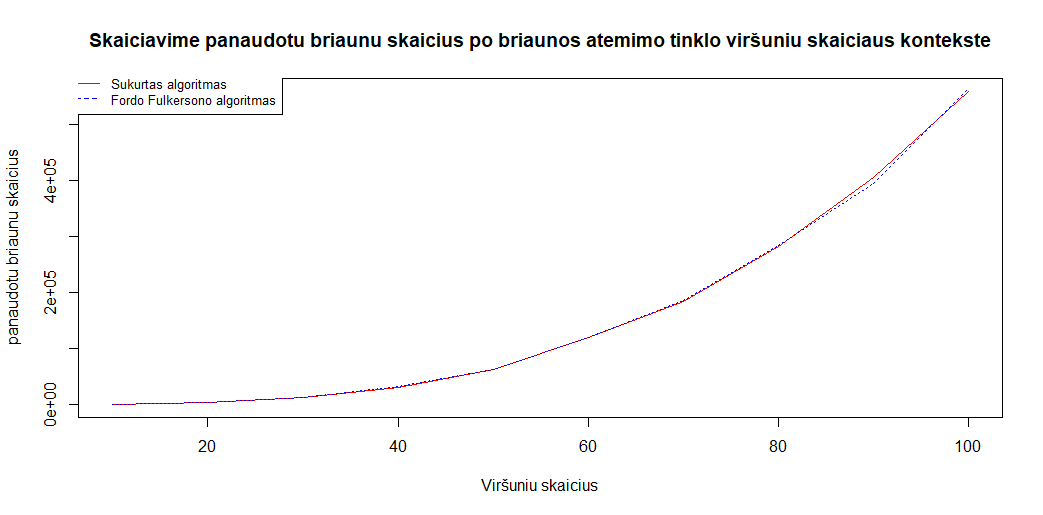
\includegraphics[width=\textwidth]{img/vre.png}
	\label{plot:vre}
\end{figure}
\begin{figure}[H]
	\caption{Skaičiavime panaudotų briaunų skaičius po briaunos talpos pakeitimo tinklo viršūnių skaičiaus kontekste}
	\centering
	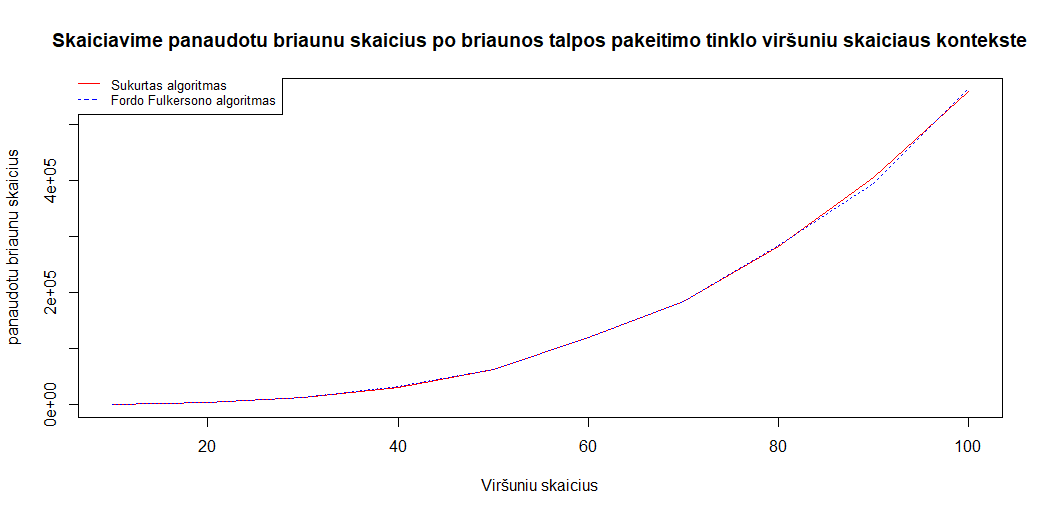
\includegraphics[width=\textwidth]{img/vue.png}
	\label{plot:vue}
\end{figure}

\begin{figure}[H]
	\caption{Skaičiavime panaudotų briaunų skaičius po viršūnės pridėjimo tinklo briaunų skaičiaus kontekste}
	\centering
	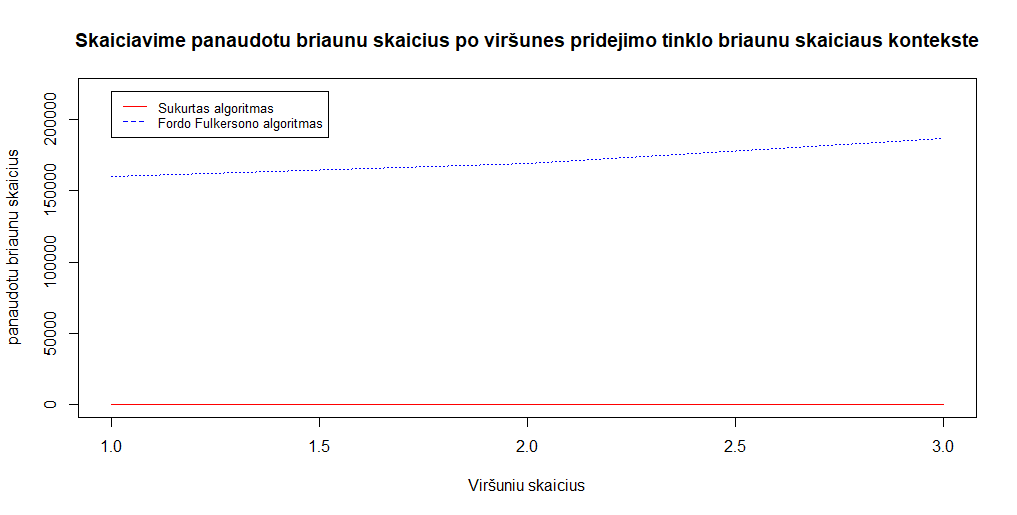
\includegraphics[width=\textwidth]{img/eav.png}
	\label{plot:eav}
\end{figure}
\begin{figure}[H]
	\caption{Skaičiavime panaudotų briaunų skaičius po briaunos pridėjimo tinklo briaunų skaičiaus kontekste}
	\centering
	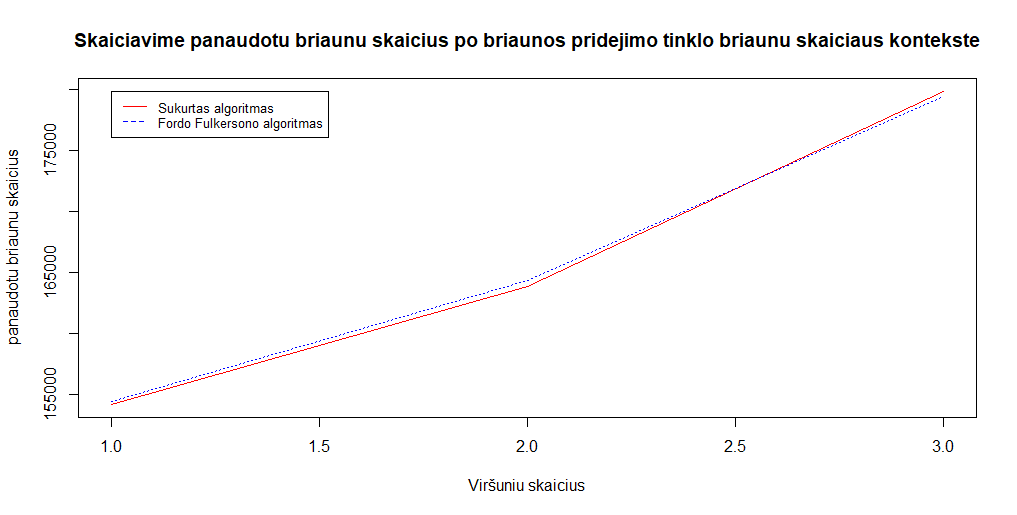
\includegraphics[width=\textwidth]{img/eae.png}
	\label{plot:eae}
\end{figure}
\begin{figure}[H]
	\caption{Skaičiavime panaudotų briaunų skaičius po viršūnės atėmimo tinklo briaunų skaičiaus kontekste}
	\centering
	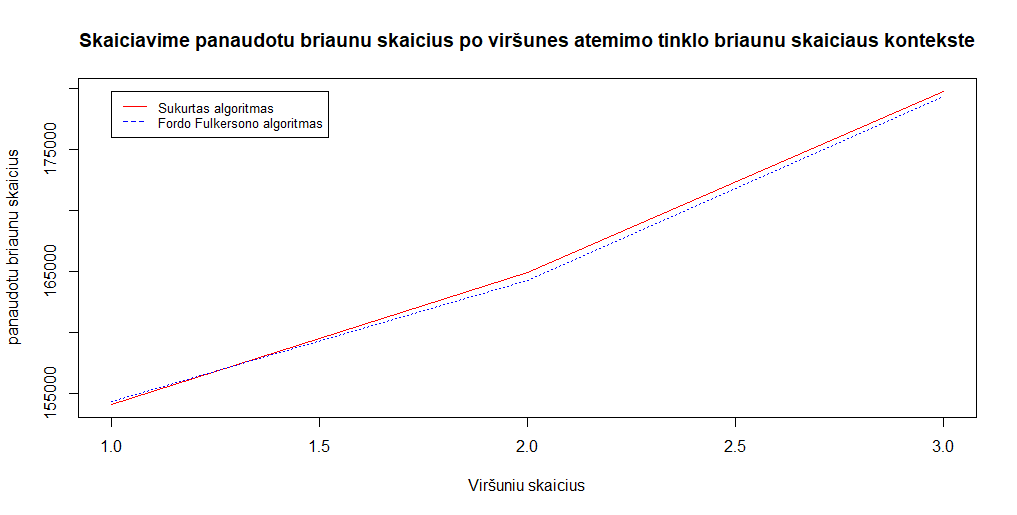
\includegraphics[width=\textwidth]{img/erv.png}
	\label{plot:erv}
\end{figure}
\begin{figure}[H]
	\caption{Skaičiavime panaudotų briaunų skaičius po briaunos atėmimo tinklo briaunų skaičiaus kontekste}
	\centering
	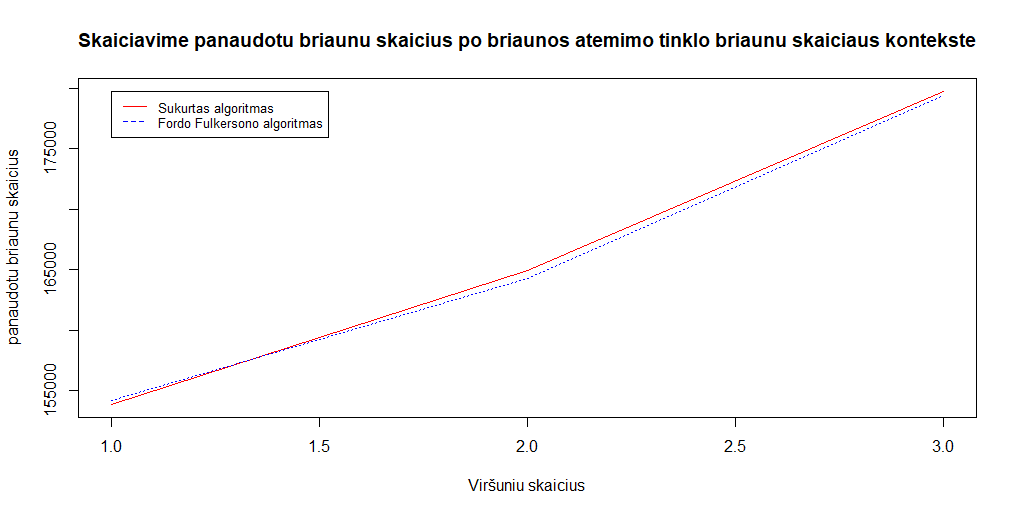
\includegraphics[width=\textwidth]{img/ere.png}
	\label{plot:ere}
\end{figure}
\begin{figure}[H]
	\caption{Skaičiavime panaudotų briaunų skaičius po briaunos talpos pakeitimo tinklo briaunų skaičiaus kontekste}
	\centering
	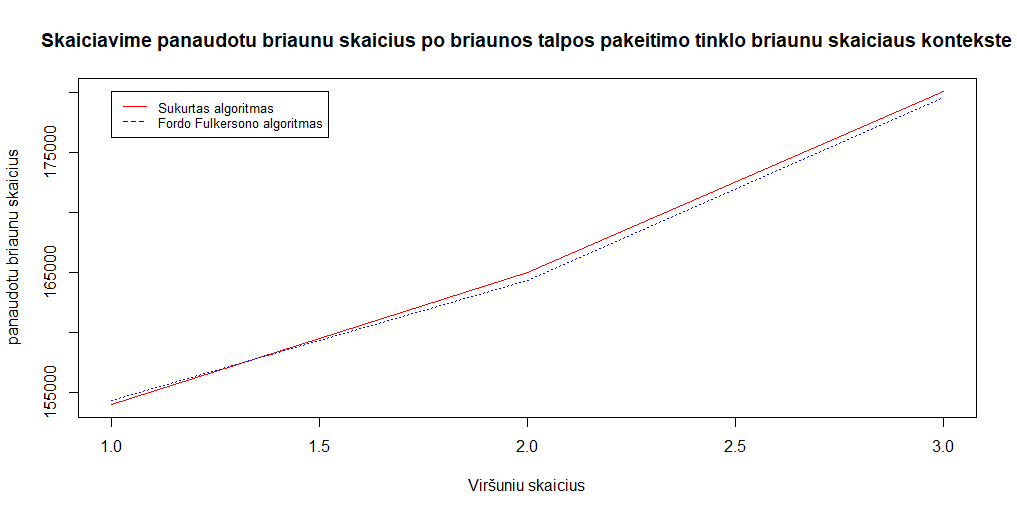
\includegraphics[width=\textwidth]{img/eue.png}
	\label{plot:eue}
\end{figure}

Naudojantis atliktų bandymų rezultatu, masyvais $Algorithm_{\{T\}}$ ir $Test_{\{T\}}$,  sukurtam algoritmui ir Fordo Fulkersono algoritmui buvo sukonstruoti paprasti linijiniai modeliai $USED\_EDGES ~ VIRSUNES + BRIAUNOS$ su kiekvienu pokyčio tipu T, kur USED\_EDGES - tai panaudotų briaunų skaičius, VIRSUNES - apskaičiuoto tinklo viršūnių skaičius, BRIAUNOS - apskaičiuoto tinklo briaunų skaičius (gali įgyti reikšmes: VIDUTINIS - vidutinis galimų briaunų skaičius, MAZAI - vidutiniškai mažesnis negu vidutinis galimų briaunų skaičius, DAUG - vidutiniškai didesnis negu vidutinis galimų briaunų skaičius). Modelių konstravimui buvo naudojamas programinis įrankis RStudio. Sukonstruoto algoritmo modeliai:
\begin{enumerate}
	\item Po viršūnės pridėjimo: $USED\_EDGES = 0$
	\item Po briaunos pridėjimo: $USED\_EDGES = 5887.2 VIRSUNES + 15967.6 DAUG - 9703.9 MAZAI + VIDUTINIS - 159948.5$, tik parametras USED\_EDGES ir konstanta turi dideles įtakas.
	\item Po viršūnės atėmimo: $USED\_EDGES = 5883.5 VIRSUNES + 14875.6 DAUG - 10817.4 MAZAI + VIDUTINIS - 158674.3$, tik parametras USED\_EDGES ir konstanta turi dideles įtakas.
	\item Po briaunos atėmimo: $USED\_EDGES = 5878.1 VIRSUNES + 14846.0 DAUG -11098.5 MAZAI + VIDUTINIS - 158368.5$, tik parametras USED\_EDGES ir konstanta turi dideles įtakas.
	\item Po talpos pakeitimo: $USED\_EDGES = 5884.8 VIRSUNES + 15084.7 DAUG - 11007.5 MAZAI + VIDUTINIS - 158659.7$, tik parametras USED\_EDGES ir konstanta turi dideles įtakas.
\end{enumerate}
Fordo Fulkersono algoritmo modeliai:
\begin{enumerate}
	\item Po viršūnės pridėjimo: $USED\_EDGES =6028.1 VIRSUNES + 17498.6 DAUG - 9517.2 MAZAI + VIDUTINIS - 162010.2$, tik parametras USED\_EDGES ir konstanta turi dideles įtakas.
	\item Po briaunos pridėjimo: $USED\_EDGES = 5870 VIRSUNES + 15070 DAUG - 9925 MAZAI + VIDUTINIS - 158514$, tik parametras USED\_EDGES ir konstanta turi dideles įtakas.
	\item Po viršūnės atėmimo: $USED\_EDGES = 5869 VIRSUNES + 15140DAUG -9863 MAZAI + VIDUTINIS - 158546$, tik parametras USED\_EDGES ir konstanta turi dideles įtakas.
	\item Po briaunos atėmimo: $USED\_EDGES = 5865.4 VIRSUNES + 15166.0 DAUG - 10081.9 MAZAI + VIDUTINIS - 158363.9$, tik parametras USED\_EDGES ir konstanta turi dideles įtakas.
	\item Po talpos pakeitimo: $USED\_EDGES = 5871.1 VIRSUNES + 15302.0 DAUG - 9947.8 MAZAI + VIDUTINIS - 158604.8$, tik parametras USED\_EDGES ir konstanta turi dideles įtakas.
\end{enumerate}

Palyginus sukurto algoritmo ir Fordo Fulkersono algoritmo paprastus linijinius modelius buvo nustatyta, kad skaičiavime panaudotų briaunų kontekste: sukurtas algoritmas yra efektyvesnis nei Frodo Fulkersono algoritmas pridedant viršūnę, visais kitais atvejais šių algoritmų efektyvumas yra apytiksliai lygus.